\documentclass{beamer}

\let\phi\varphi
\newcommand{\field}{\mathbf{F}}
\newcommand{\impliesn}[1]{\underset{#1}{\implies}}
\newcommand{\iffn}[1]{\underset{#1}{\iff}}
\newcommand{\impliesp}{\impliesn{p}}
\newcommand{\iffp}{\iffn{p}}
\newcommand{\impliespp}{\impliesn{p'}}
\newcommand{\iffpp}{\iffn{p'}}
\newcommand{\ex}{\mathbf{E}}


\mode<presentation>
{
\usetheme{default}
}
\setbeamertemplate{navigation symbols}{}
\usecolortheme[rgb={0.13,0.28,0.59}]{structure}
\setbeamertemplate{itemize subitem}{--}
\setbeamertemplate{frametitle} {
        \begin{center}
          {\large\bf \insertframetitle}
        \end{center}
}

\newcommand\footlineon{
  \setbeamertemplate{footline} {
    \begin{beamercolorbox}[ht=2.5ex,dp=1.125ex,leftskip=.8cm,rightskip=.6cm]{structure}
      \footnotesize \insertsection
      \hfill
      {\insertframenumber}
    \end{beamercolorbox}
    \vskip 0.45cm
  }
}
\footlineon

\AtBeginSection[]
{       
        \begin{frame}<beamer> 
                \frametitle{Outline} 
                \tableofcontents[currentsection,currentsubsection]
        \end{frame}
}

% \usepackage{subcaption}
\usepackage{amsmath,amssymb,amsthm}
\usepackage{xcolor}
\usepackage{graphicx}
\usepackage{tikz}
\usetikzlibrary{matrix, positioning}

\newcommand{\blue}[1]{{\color{blue}#1}}
\newcommand{\red}[1]{{\color{red}#1}}

\makeatletter
\def\mathcolor#1#{\@mathcolor{#1}}
\def\@mathcolor#1#2#3{%
  \protect\leavevmode
  \begingroup
    \color#1{#2}#3%
  \endgroup
}
\makeatother

\title{Vector Subspace Structure and FRI}
\author{Guillermo Angeris \and Alex Evans}
\date{Session 3, SPLA Study Club}

\newcommand{\ones}{\mathbf 1}
\newcommand{\reals}{{\mbox{\bf R}}}
\newcommand{\integers}{{\mbox{\bf Z}}}
\newcommand{\symm}{{\mbox{\bf S}}}  % symmetric matrices

\newcommand{\nullspace}{{\mathcal N}}
\newcommand{\range}{{\mathcal R}}
\newcommand{\Rank}{\mathop{\bf Rank}}
\newcommand{\tr}{\mathop{\bf tr}}
\newcommand{\diag}{\mathop{\bf diag}}
\newcommand{\card}{\mathop{\bf card}}
\newcommand{\rank}{\mathop{\bf rank}}
\newcommand{\conv}{\mathop{\bf conv}}
\newcommand{\prox}{\mathbf{prox}}

\newcommand{\Expect}{\mathop{\bf E{}}}
\newcommand{\Prob}{\mathop{\bf Prob}}
\newcommand{\Co}{{\mathop {\bf Co}}} % convex hull
\newcommand{\dist}{\mathop{\bf dist{}}}
%\newcommand{\argmin}{\mathop{\rm argmin}}
%\newcommand{\argmax}{\mathop{\rm argmax}}
\DeclareMathOperator*{\argmin}{argmin}
\DeclareMathOperator*{\argmax}{argmax}
\newcommand{\epi}{\mathop{\bf epi}} % epigraph
\newcommand{\Vol}{\mathop{\bf vol}}
\newcommand{\dom}{\mathop{\bf dom}} % domain
\newcommand{\intr}{\mathop{\bf int}}
\newcommand{\sign}{\mathop{\bf sign}}

\newcommand{\cf}{{\it cf.}}
\newcommand{\eg}{{\it e.g.}}
\newcommand{\ie}{{\it i.e.}}
\newcommand{\etc}{{\it etc.}}

\newcommand{\BEAS}{\begin{eqnarray*}}
\newcommand{\EEAS}{\end{eqnarray*}}
\newcommand{\BEA}{\begin{eqnarray}}
\newcommand{\EEA}{\end{eqnarray}}
\newcommand{\BEQ}{\begin{equation}}
\newcommand{\EEQ}{\end{equation}}
\newcommand{\BIT}{\begin{itemize}}
\newcommand{\EIT}{\end{itemize}}

\begin{document}
	\begin{frame}
		\titlepage
	\end{frame}
	
    \section{Overview}
    \begin{frame}
        \frametitle{Quick recap}
        \begin{itemize}\itemsep=12pt
            \item We've studied all main tools necessary
            \item And most of the major checks
            \item (Either via homework or lecture!)
            \item Now, we're going to do something real with them!
        \end{itemize}
	\end{frame}

    \begin{frame}
        \frametitle{Main idea}
        \begin{itemize}\itemsep=12pt
            \item The main point will be to try and understand FRI
            \item To do this, we need some FRI-specific set up
            \item Namely: decomposing a vector space recursively
            \pause
            \item Similar to previous: start with exact case
            \item Move to inexact case (which is `harder')
        \end{itemize}
	\end{frame}

    \section{Vector subspaces}
    \begin{frame}
        \frametitle{Subspaces and decomposition}
        \begin{itemize}\itemsep=12pt
            \item We start back with subspaces
            \item Let $V \subseteq \field^n$ be a subspace (along with $V', V'' \subseteq \field^n$)
            \item We say $V$ \emph{decomposes} into $V'$ and $V''$ if, for each $x \in V$,
            \[
                x = y + z,
            \]
            for some $y \in V'$ and $z \in V''$
            \item We write this as
            \[
                V = V' + V''
            \]
        \end{itemize}
	\end{frame}

    \begin{frame}
        \frametitle{An example}
        \begin{itemize}\itemsep=12pt
            \item A simple example: let $V = \field^2$, then
            \[
                V = \{(\alpha, 0) \mid \alpha \in \field\} + \{(0, \beta) \mid \beta \in \field\}
            \]
        \end{itemize}
	\end{frame}

    \begin{frame}
        \frametitle{A (more complicated) example}
        \begin{itemize}\itemsep=12pt
            \item A second example is: let $V$ be the Reed--Solomon codewords
            \[
                V = \{(f(\alpha_1), \dots, f(\alpha_m)) \mid \text{$f$ has degree $\le n-1$}\}
            \]

            \pause

            \item If we define the following subspaces (check this!)
            \[
                \begin{aligned}
                    V' &= \{(f(\alpha_1), \dots, f(\alpha_m)) \mid \text{$f$ has \blue{even} powers, deg.\ $\le n-1$}\}\\
                    V'' &= \{(f(\alpha_1), \dots, f(\alpha_m)) \mid \text{$f$ has \red{odd} powers, deg.\ $\le n-1$}\}
                \end{aligned}
            \]

            \item Then
            \[
                V = V' + V''
            \]
        \end{itemize}
	\end{frame}


    \begin{frame}
        \frametitle{Not a difficult observation}
        \begin{itemize}\itemsep=12pt
            \item Note that, if $n$ is even
            \[
                f(\alpha) = \blue{x_1} + \red{x_2\alpha} + \blue{x_3\alpha^2} + \dots + \red{x_n \alpha^{n-1}}
            \]

            \pause

            \item Same as saying:
            \[
                f(\alpha) = \underbrace{\blue{x_1} + \blue{x_3\alpha^2} + \blue{\dots}}_\text{even powers}
                    + \underbrace{\red{x_2\alpha} + \red{x_4\alpha^3} + \red{\dots}}_\text{odd powers}
            \]
        \end{itemize}
	\end{frame}

    \begin{frame}
        \frametitle{Recursive decomposition}
        \begin{itemize}\itemsep=12pt
            \item Given a vector space $V\subseteq \field^{n}$ and a matrix $T\in
                \field^{m \times n}$, then
            \[
                TV = \{Tx \mid x \in V\}
            \]
            is also a vector space

            \pause

            \item (Homework problem!)

            \pause

            \item We say this subspace \emph{recursively decomposes} if 
            \[
                V = T_1V' + T_2V',
            \]
            for $V' \subseteq \field^{k}$ and $T_1, T_2 \in \field^{n \times k}$
        \end{itemize}
	\end{frame}

    \begin{frame}
        \frametitle{Simple example}
        \begin{itemize}\itemsep=12pt
            \item Same example as before! If $V = \field^2$, then
            \[
                V = \begin{bmatrix} 1\\0 \end{bmatrix}\field + \begin{bmatrix} 0\\1 \end{bmatrix}\field
            \]

            \pause

            \item Or, more generally, if $V=\field^{2n}$, then
            \[
                V = \begin{bmatrix} I\\0 \end{bmatrix}\field^n + \begin{bmatrix} 0\\I \end{bmatrix}\field^n 
            \]
            (See homework!)
        \end{itemize}
	\end{frame}

    \begin{frame}
        \frametitle{Reed--Solomon example}
        \begin{itemize}\itemsep=12pt
            \item From before, let $V$ be the Reed--Solomon codewords, $n$ even
            \[
                V = \{(f(\alpha_1), \dots, f(\alpha_m)) \mid \text{$f$ has degree $\le n-1$}\}
            \]

            \item And define (as before)
            \[
                V' = \{(f(\alpha_1), \dots, f(\alpha_m)) \mid \text{$f$ has \blue{even} powers, deg.\ $\le n-1$}\}
            \]

            \pause

            \item Then, $V$ can be written $V = V' + DV'$, where
            \[
                D = \begin{bmatrix}
                        \alpha_1 & 0 & \dots & 0\\
                        0 & \alpha_2 & \dots & 0\\
                        \vdots & \vdots & \ddots & \vdots\\
                        0 & 0 & \dots & \alpha_m
                    \end{bmatrix}
            \]
            (See homework!)
        \end{itemize}
	\end{frame}

    \section{An exact subspace check}
    \begin{frame}
        \frametitle{How do we use this?}
        \begin{itemize}\itemsep=12pt
            \item Clearly, these spaces have a lot of structure
            \item How can we use it?
            \pause
            \item Let's design a (simple?) protocol!
        \end{itemize}
	\end{frame}

    \begin{frame}
        \frametitle{A simple check}
        \begin{itemize}\itemsep=12pt
            \item Want to check if $x \in V$ when $V = T_1V' + T_2V'$
            \pause
            \item Suffices to check that
            \begin{enumerate}\itemsep=8pt
                \item The equality $x = T_1y+T_2z$ holds
                \item Subspace inclusion is satisfied: $y, z \in V'$
            \end{enumerate}
            \pause
            \item Savings if checking that $y, z \in V'$ takes at least $\sim n^2$ time
            \pause
            \item If $V'$ decomposes further, then more savings!
        \end{itemize}
	\end{frame}

    \begin{frame}
        \frametitle{Where is the randomness?}
        \begin{itemize}\itemsep=12pt
            \item From before, let $G \in \field^{m \times 2}$ with distance $d$
            \item Remembering the vector subspace check from session 2:
            \[
                G_{r1}y + G_{r2}z \in V' \impliesp y, z \in V',
            \]
            where $p \le 1-d/m$
            \item With this additional step, we have a protocol with error $\le p$
            \begin{enumerate}\itemsep=8pt
                \item Check equality $x = T_1y+T_2z$ holds
                \item Draw random $r$ from $1, \dots, m$
                \item Verify that $G_{r1}y + G_{r2}z \in V'$
            \end{enumerate}
        \end{itemize}
	\end{frame}

    \begin{frame}
        \frametitle{Where is the randomness?}
        \begin{itemize}\itemsep=12pt
            \item Protocol from before:
            \begin{enumerate}\itemsep=8pt
                \item Check equality $x = T_1y+T_2z$ holds
                \item Draw random $r$ from $1, \dots, m$
                \item Verify that $G_{r1}y + G_{r2}z \in V'$
            \end{enumerate}
            \item Why does this imply that $x \in V$ with error probability $\le p$?
        \end{itemize}
	\end{frame}

    \section{A subspace distance check}
    \begin{frame}
        \frametitle{Exact checks}
        \begin{itemize}\itemsep=12pt
            \item Note that the previous `protocol' requires exact equality
            \item (And exact inclusion!)
            \pause
            \item Hard to achieve unless we are in the coding model
            \item For the same reason as the exact zero check
        \end{itemize}
	\end{frame}

    \begin{frame}
        \frametitle{Distance check}
        \begin{itemize}\itemsep=12pt
            \item On the other hand, say we're in the direct access model
            \item How can we relax these conditions?
            \pause
            \item First, relax exact equality to `close enough'
            \pause
            \item Second, relax exact inclusion to `close enough' :)
            \pause
            \item What does this mean?
        \end{itemize}
	\end{frame}

    \begin{frame}
        \frametitle{Distance to a subspace}
        \begin{itemize}\itemsep=12pt
            \item As usual, distance between two vectors $x, y \in \field^n$ is defined
            \[
                \|x - y\|_0
            \]
            \item (This is easy-ish via sparsity check! See previous homework)
            \pause
            \item Given a subspace $V\subseteq \field^n$, the \emph{distance} of $x$ to $V$ is
                written
            \[
                \|x - V\|_0 = \min_{y \in V} \|x - y\|_0
            \]
        \end{itemize}
	\end{frame}

    \begin{frame}
        \frametitle{Matrix distance}
        \begin{itemize}\itemsep=12pt
            \item Given a matrix $X$, we say
            \[
                \Delta(X, V) \le q
            \]
            if there is a matrix $Y$, with columns in $V$, such that $X - Y$ has at most $q$ nonzero rows (mouthful!)
            \pause
            \item The picture is
            \begin{figure}
                \centering
                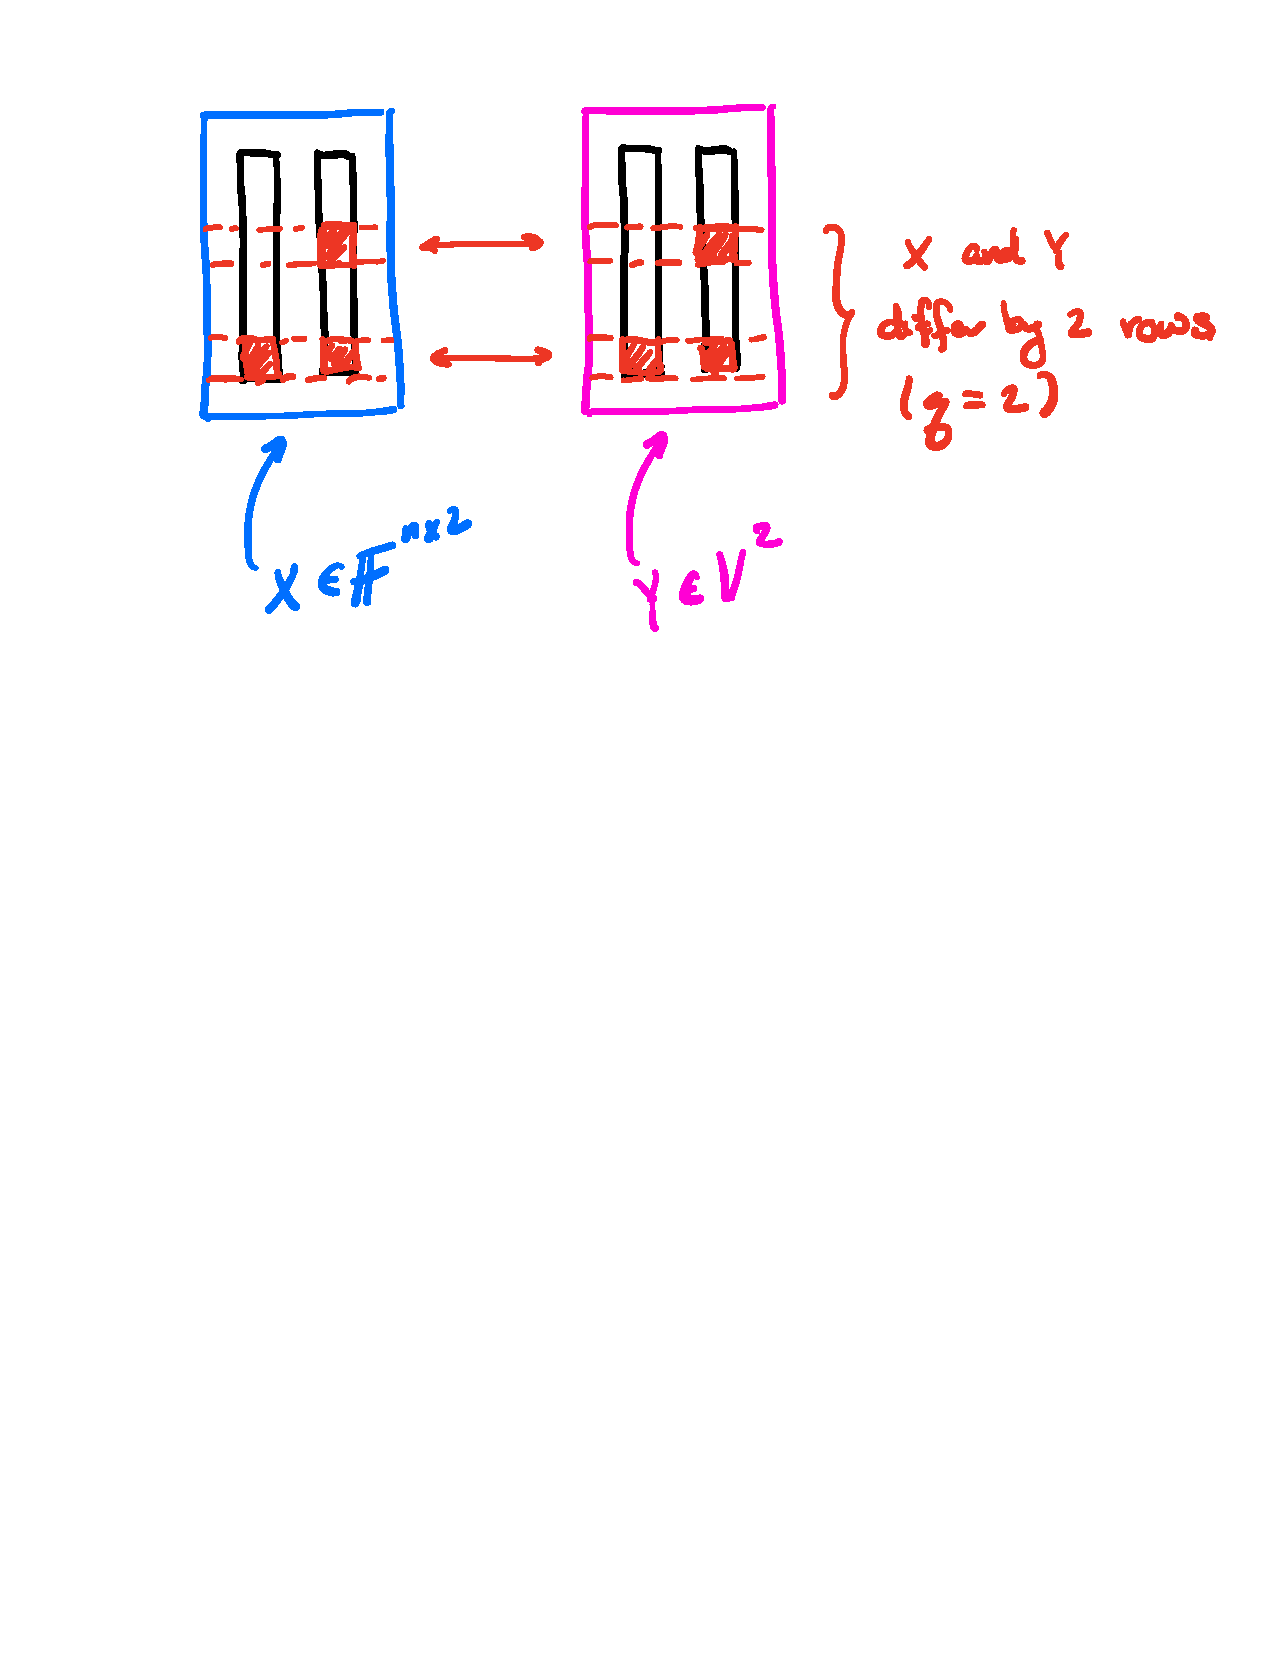
\includegraphics[clip, trim=0 7in 0 .5in, width=.8\textwidth]{figures/mat-distance.pdf}
            \end{figure}
        \end{itemize}
	\end{frame}

    \begin{frame}
        \frametitle{Revised protocol}
        \begin{itemize}\itemsep=12pt
            \item Start with a simple revision: let $q$ be an `acceptable distance'
            \begin{enumerate}\itemsep=8pt
                \item Check that $\|x - (T_1y + T_2z)\|_0 \le q$
                \item Draw random $r$ from $1, \dots, m$
                \item Check that $\|G_{r1}y + G_{r2}z - V'\|_0 \le q$
            \end{enumerate}
            \item Does this guarantee that $\|x - V\| \le Cq$ for some $C$?
            \pause
            \item Remember, $T_1$ and $T_2$ can be very badly structured!
        \end{itemize}
	\end{frame}

    \begin{frame}
        \frametitle{Structure on $T_i$}
        \begin{itemize}\itemsep=12pt
            \item Unfortunately, sparsity depends on structure
            \pause
            \item We need one more definition: $T_1$ and $T_2$ are \emph{basis aligned}
            \item Whenever $[y~z]$ has $\le q$ nonzero rows, then
            \[
                T_1y + T_2z
            \]
            has $\le q'$ nonzero entries
            \pause
            \item Example: $q = q'$ if $T_1$ and $T_2$ are only diagonal (see homework!)
        \end{itemize}
	\end{frame}

    \begin{frame}
        \frametitle{High level of basis alignment}
        \begin{itemize}\itemsep=12pt
            \item Essentially, basis alignment means if $y$ and $z$ are $q$-close to $V'$
            \item Then, we have that $T_1y + T_2z$ must be $q'$-close to $V$
            \item And this is the last step we need!
        \end{itemize}
	\end{frame}

    \begin{frame}
        \frametitle{(One step of) the FRI protocol}
        \begin{itemize}\itemsep=12pt
            \item Let $V$ be the set of Reed--Solomon codes of degree $2k$
            \item And $V'$ is the same set with degree $k$ (instead of $2k$)
            \item Note that protocol is
            \begin{enumerate}\itemsep=8pt
                \item Check that $\|x - (T_1y + T_2z)\|_0 \le q$
                \item Draw random $r$ from $1, \dots, m$
                \item Check that $\|G_{r1}y + G_{r2}z - V'\|_0 \le q$
            \end{enumerate}
            \pause
            \item First is a sparse check, third is a subspace distance check
            \item Implies that $\|x - V\|_0 \le 2q$ (with some probability)
        \end{itemize}
	\end{frame}
    \begin{frame}
        \frametitle{Recursive application}
        \begin{itemize}\itemsep=12pt
            \item Since $V'$ is also an RS code, then it too decomposes!
            \item Instead of checking the last step
            \[
                \|G_{r1}y + G_{r2}z - V'\|_0 \le q
            \]
            \item Run the protocol again, over new vector
            \[
                w = G_{r1}y + G_{r2}z
            \]
            
            \pause
            \item Terminate at some later point by just checking inclusion
        \end{itemize}
	\end{frame}
    \begin{frame}
        \frametitle{Result}
        \begin{itemize}\itemsep=12pt
            \item If we repeat this $k$ times, we get that
            \[
                \|x - V\| \le 2q
            \]
            with high probability
            \item The details are a bit messy (though ultimately easy)
            \item See paper~\S4.2
        \end{itemize}
	\end{frame}

    \begin{frame}
        \frametitle{High level result}
        \begin{itemize}\itemsep=12pt
            \item We started with checking $x$ close to $V$
            \item Reduced it to getting $y$ and $z$ which have two properties
            \pause
            \item First, $T_1y + T_2z$ is close to $x$
            \pause
            \item Second $y$ and $z$ are each close to $V'$
            \item `Reduce' this further to checking $G_{r1}y + G_{r2}z$ is close to $V'$
            \pause
            \item And then iterate!
        \end{itemize}
	\end{frame}

    \begin{frame}
        \frametitle{High level discussion}
        \begin{itemize}\itemsep=12pt
            \item Note that polynomials aren't really needed
            \item But they make a \emph{great} practical case
            \item (Possible that there may be structured codes that are useful)
        \end{itemize}
	\end{frame}

    \section{Conclusion}
    \begin{frame}
        \frametitle{La fin}
        \begin{itemize}\itemsep=12pt
            \item With all of that; we have `finished' the course
            \item Many tools, one example application, but likely many more
            \item Encourage you to go and try to write others using this!
            \item Please PR for homework and slide feedback if needed :)
            \pause
            \item And thanks for attending!
        \end{itemize}
	\end{frame}
\end{document}
